

\section{Overview and Key Ideas}
\label{sec:overview}


In this section, we provide a brief outline of the basics of
Separation Logic (SL) and its inductive predicates. Next, we explain
how to use the existing ILP system \popper~\cite{cropper2021learning}
to synthesise such predicates from \emph{both positive and negative}
examples, and how we handle with learning from positive examples only.
%
We conclude with the high-level workflow of our SL predicate
synthesiser \tool.

\subsection{Inductive Predicates in Separation Logic}
\label{sec:sl}

\begin{figure}
  \centering
%  \belowcaptionskip=-10pt
%  \abovecaptionskip=5pt
  \includegraphics[width=0.8\textwidth]{figure/sll.pdf}
% \setlength{\abovecaptionskip}{0pt}

  \caption{Memory layout of a singly linked list.}
  \label{fig:sll}
\end{figure}
% 
Consider a schematic memory layout depicted in \autoref{fig:sll}
corresponding to a singly linked list (SLL).
%
The list has a recurring structure with each of its elements
represented by a consecutive pair of memory locations (the ``head''
one referred to by a pointer variable~\code{x}), the first one storing
its data value (or \emph{payload})~\code{v} and the second containing
the address \code{y} of the tail of the list. 
%
Knowing these shape constraints, the entire list can be traversed
recursively by starting from the head and following the tail pointers.
% thus, getting access to its payload.


The idea of defining the repetitive shape of a heap-based linked
structure, such as SLL, is precisely captured by Separation Logic and
its inductive (\ie, well-founded recursive) predicates. One encoding
of an SLL heap shape via the SL predicate \code{sll} is given below:

% The idea of defining the repetitive shape of heap-based linked
% structures
% %, such as SLL,  %for page break reason
% is captured by Separation Logic and
% its inductive (\ie, well-founded recursive) predicates. One
% encoding
% of an SLL heap shape   is given via the SL predicate:

\begin{lstlisting}
  pred sll(loc x, set s) where
    | x = 0 $\Rightarrow$ { s = {}; emp }
    | x $\neq$ 0 $\Rightarrow$ { s = {v} $\cup$ s1; x $\mapsto$ v * (x+1) $\mapsto$ y * sll(y, s1) }
\end{lstlisting}

\noindent
%
The predicate \code{sll} is parameterised by a location (\ie, pointer variable)
\code{x} and a payload set of the data structure
\code{s};
%
% \is{We could use algebraic lists to encode payloads instead of sets.
%   We should either address it or explain our choice.}
%
it holds true for any
\emph{heap fragment} that follows the shape of a linked list (and
contains no extra heap space).
%
What exactly that shape is, is defined by the two \emph{clauses} (\aka
constructors) of the predicate. 
%
The first one handles the case when \code{x} is a null-pointer,
constraining the payload set \code{s} of the list to be empty
(\code{\{\}}); the same holds for the list-carrying heap---which is
denoted by a standard SL assertion \code{emp}.\footnote{For
  simplicity, our examples use mathematical sets to encode the data
  payload, assuming uniqueness of the elements, instead of, \eg, an
  algebraic list. This is not a conceptual or practical limitation of
  our approach, as we will show in \autoref{sec:done}.}
%
The second clause describes a more interesting case, in which \code{x}
is not null, and so the payload can be split to an element \code{v}
and the residual payload \code{s1} (for simplicity of this example, we
assume that all elements of the list are unique).
%
Furthermore, the heap carrying the list is specified to have two
consecutive locations, \code{x} and \code{x + 1}, storing \code{v}
and some (existentially quantified) pointer value \code{y}, as denoted
by the SL \emph{points-to} notation $\mapsto$.
%
Finally, the rest of the SLL-carrying heap is 
the recursive occurrence of the same predicate \code{sll(y, s1)} (with
different arguments), thus replicating the recursive structure of the
layout from \autoref{fig:sll}.
%
% The heap-related constraints appearing after the semicolon in the
% clauses are traditionally referred to as \emph{spatial},
% while the remaining constraints (such as, \eg, the statement \code{s
%   == \{\}} constraining the empty list payload) are usually called
% \emph{pure}.



The logical connective \code{*} appearing in the second clause of the
\code{sll} predicate is known as the \emph{separating conjunction}
(sometimes pronounced ``and separately'') and is the main enabling
feature of Separation Logic~\cite{OHearn-al:CSL01}.
%
It implicitly constrains the symbolic heaps it connects in a spatial
assertion to have \emph{disjoint} domains.
%
Specifically, in this example it implies that the heap fragment
captured by \code{sll(y, s1)} does not contain memory locations
referred to by either \code{x} or \code{x+1}.
%
Such disjointness constraint  is what makes it
possible to avoid extensive reasoning about aliasing when using SL
specifications, making them \emph{modular}, \ie, holding true in the
context of any heap that is larger than what is affected by the
specified program.
%


% \subsection{\popper an ASP-based ILP system}

% \pagebreak

% \vspace{-5pt}
  
\subsection{From  Memory Graphs to Heap Predicates}
% \subsection{Synthesising Heap Predicates via ILP} maybe?
\label{sec:popper}

Our goal is to synthesise inductive SL predicates from examples of
concrete memory graphs.
%
To do so, we phrase both SL predicates and the memory graphs that
satisfy them in terms of Logic Programming. For example, the \prolog
predicate below defines a sorted singly linked list:
%
\begin{minted}[fontsize=\small]{prolog}
  srtl(X, S) :- empty(S), nullptr(X).
  srtl(X, S) :- next(X,Y), value(X,V), srtl(Y,SY), min_set(V,S), insert(SY,V,S).
\end{minted}
%
The predicate above defines a sorted singly linked list by enhancing
the ordinary singly linked list predicate with the constraint
\pcode{min_set(V, S)} that states that the value \pcode{V} is equal to
the smallest value in the set \pcode{S}. The \pcode{insert(S1, V, S)}
and \pcode{empty(S)} (\ie, \pcode{s == {v} ++ s1} and \pcode{s == {}}
in the SLL example) are defined using \prolog built-in predicates that
correspond to ordinary functions in set theory.
%
Other \prolog-style predicates used in the synthesised SL solutions
are data-structure specific and are extracted from the user-provided
memory graphs.
%
We leave till later (\autoref{sec:sldomain}) the issue of ensuring
that a \prolog predicate is also a \emph{valid} SL predicate in the
sense that it does not use SL connectives in a contradictory way,
allowing one to derive falsehood from its definition.


%
% Most of the predicates contributing to the definition of \code{srtl}
% come from predefined vocabularies, which the synthesiser will be aware
% of. During the search, it will be looking for definitions that can fix
% a number of clauses and combine available constraints, using the
% user-provided examples to validate its guesses.
%

\begin{figure}[t]
%\vspace{-15pt}
\centering
% \scalebox{0.75}{{\small{
\begin{tabular}{c}
    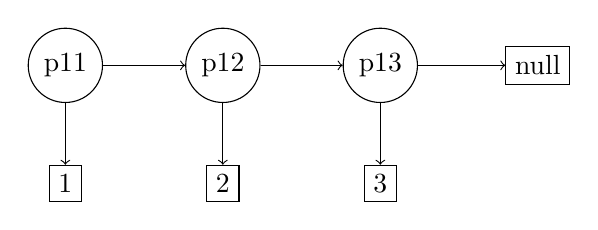
\begin{tikzpicture}
        \node[circle, draw] (n1) at (0,1.5) {p11};
        \node[circle, draw] (n2) at (2,1.5) {p12};
        \node[circle, draw] (n3) at (4,1.5) {p13};
        \node[draw] (null) at (6,1.5) {null};
        \node[draw] (v1) at (0,0) {1};
        \node[draw] (v2) at (2,0) {2};
        \node[draw] (v3) at (4,0) {3};
        \draw[->] (n1) --  node [above,midway] {\mynext} (n2);
        \draw[->] (n2) --  node [above,midway] {\mynext} (n3);
        \draw[->] (n3) --  node [above,midway] {\mynext} (null);
        \draw[->] (n1) --  node [midway] [above,midway,sloped] {\myvalue} (v1);
        \draw[->] (n2) --  node [midway] [above,midway,sloped] {\myvalue} (v2);
        \draw[->] (n3) --  node [midway] [above,midway,sloped] {\myvalue} (v3);
    \end{tikzpicture}
\\
\\
  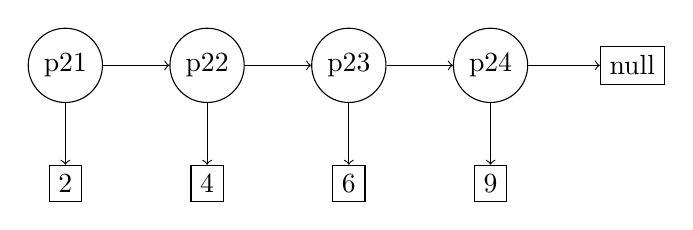
\begin{tikzpicture}
        \node[circle, draw] (n1) at (0,1.5) {p21};
        \node[circle, draw] (n2) at (1.8,1.5) {p22};
        \node[circle, draw] (n3) at (3.6,1.5) {p23};
        \node[circle, draw] (n4) at (5.4,1.5) {p24};
        \node[draw] (null) at (7.2,1.5) {null};
        \node[draw] (v1) at (0,0) {2};
        \node[draw] (v2) at (1.8,0) {4};
        \node[draw] (v3) at (3.6,0) {6};
        \node[draw] (v4) at (5.4,0) {9};
        \draw[->] (n1) --  node [above,midway] {\mynext} (n2);
        \draw[->] (n2) --  node [above,midway] {\mynext} (n3);
        \draw[->] (n3) --  node [above,midway] {\mynext} (n4);
        \draw[->] (n4) --  node [above,midway] {\mynext} (null);
        \draw[->] (n1) --  node [above,midway,sloped] {\myvalue} (v1);
        \draw[->] (n2) --  node [above,midway,sloped] {\myvalue} (v2);
        \draw[->] (n3) --  node [above,midway,sloped] {\myvalue} (v3);
        \draw[->] (n4) --  node [above,midway,sloped] {\myvalue} (v4);
    \end{tikzpicture}
\end{tabular}
}}
}
{\small{
\begin{tabular}{c}
    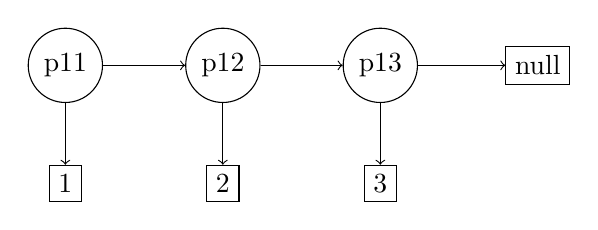
\begin{tikzpicture}
        \node[circle, draw] (n1) at (0,1.5) {p11};
        \node[circle, draw] (n2) at (2,1.5) {p12};
        \node[circle, draw] (n3) at (4,1.5) {p13};
        \node[draw] (null) at (6,1.5) {null};
        \node[draw] (v1) at (0,0) {1};
        \node[draw] (v2) at (2,0) {2};
        \node[draw] (v3) at (4,0) {3};
        \draw[->] (n1) --  node [above,midway] {\mynext} (n2);
        \draw[->] (n2) --  node [above,midway] {\mynext} (n3);
        \draw[->] (n3) --  node [above,midway] {\mynext} (null);
        \draw[->] (n1) --  node [midway] [above,midway,sloped] {\myvalue} (v1);
        \draw[->] (n2) --  node [midway] [above,midway,sloped] {\myvalue} (v2);
        \draw[->] (n3) --  node [midway] [above,midway,sloped] {\myvalue} (v3);
    \end{tikzpicture}
\\
\\
  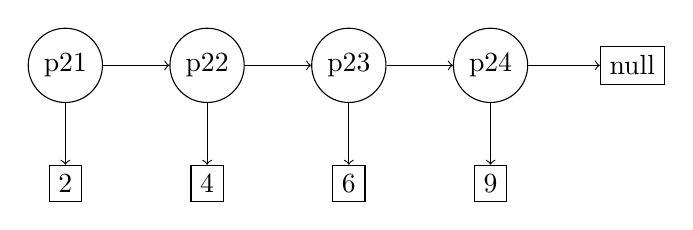
\begin{tikzpicture}
        \node[circle, draw] (n1) at (0,1.5) {p21};
        \node[circle, draw] (n2) at (1.8,1.5) {p22};
        \node[circle, draw] (n3) at (3.6,1.5) {p23};
        \node[circle, draw] (n4) at (5.4,1.5) {p24};
        \node[draw] (null) at (7.2,1.5) {null};
        \node[draw] (v1) at (0,0) {2};
        \node[draw] (v2) at (1.8,0) {4};
        \node[draw] (v3) at (3.6,0) {6};
        \node[draw] (v4) at (5.4,0) {9};
        \draw[->] (n1) --  node [above,midway] {\mynext} (n2);
        \draw[->] (n2) --  node [above,midway] {\mynext} (n3);
        \draw[->] (n3) --  node [above,midway] {\mynext} (n4);
        \draw[->] (n4) --  node [above,midway] {\mynext} (null);
        \draw[->] (n1) --  node [above,midway,sloped] {\myvalue} (v1);
        \draw[->] (n2) --  node [above,midway,sloped] {\myvalue} (v2);
        \draw[->] (n3) --  node [above,midway,sloped] {\myvalue} (v3);
        \draw[->] (n4) --  node [above,midway,sloped] {\myvalue} (v4);
    \end{tikzpicture}
\end{tabular}
}}

\\[5pt]
\begin{minted}[fontsize=\small]{prolog}
  pos(srtl(p11,[1,2,3])). pos(srtl(p21,[2,4,6,9])).

  % Encoding of the first memory graph from Fig.2
  next(p11, p12). next(p12, p13). next(p13, null). 
  value(p11, 1).  value(p12, 2).  value(p13, 3).

  % Encoding of the second memory graph from Fig.2
  next(p21, p22). next(p22, p23). next(p23, p24). next(p24, null).
  value(p21, 2).  value(p22, 4).  value(p23, 6).  value(p24, 9).
\end{minted}

%\setlength{\abovecaptionskip}{5pt}
% \setlength{\belowcaptionskip}{-10pt}
    \caption{Positive examples of sorted list heap graphs, with the corresponding logic encoding.}
    \label{fig:sorted-list}
\end{figure}

The top of \autoref{fig:sorted-list} shows two memory graphs of sorted
lists that can be used to synthesise \pcode{srtl()}.
%
For a more natural representation in terms of Logic Programming, we
use Java-style naming of structure components, \ie, fields such as
{\small{\textsf{value}}} and {\small{\textsf{next}}} instead of
C-style integer pointer offsets;
%
these fields provide the data-specific predicates (\ie, \pcode{next()}
and \pcode{value()}) to the synthesiser. In the bottom of
\autoref{fig:sorted-list}, we provide the corresponding logic
representations of the inputs to the synthesiser, consisting of
positive examples (\ie, instances of the sought predicate that are
expected to be true), and the background knowledge (\ie, encoding of
the corresponding memory graphs) that should be used to derive those
examples using predicate candidates.
%
Given all this information, a synthesiser should be able to generate
the predicate \pcode{srtl()} that satisfies the positive examples.
%
That is, using the traditional program synthesis from
input-output pairs as an analogy~\cite{GulwaniPS17}, the facts in
background knowledge (\eg, \pcode{next(p11, p12)}) are inputs, the
examples (\eg, \pcode{pos(srtl(p11, [1,2,3]))}) are the outputs, and
the solution is the program (\ie, the predicate) to be synthesised.

% \begin{figure}[t]
% % \setlength{\belowcaptionskip}{-10pt}
% % \setlength{\abovecaptionskip}{5pt}
% \begin{minted}[fontsize=\small]{prolog}
%   pos(srtl(p11,[1,2,3])). pos(srtl(p21,[2,4,6,9])).

%   % Encoding of the first memory graph from Fig.2
%   next(p11, p12). next(p12, p13). next(p13, null). 
%   value(p11, 1).  value(p12, 2).  value(p13, 3).

%   % Encoding of the second memory graph from Fig.2
%   next(p21, p22). next(p22, p23). next(p23, p24). next(p24, null).
%   value(p21, 2).  value(p22, 4).  value(p23, 6).  value(p24, 9).
% \end{minted}
% \caption{Positive examples for \code{srtl} in \popper. \todo{merge to one figure?}}
% \label{fig:examples}
% \end{figure}


\subsection{Predicate Synthesis via Answer Set Programming}
\label{sec:asp}

We observe that the synthesis of SL predicates can be regarded as a
Logic Programming synthesis task, studied extensively in the field of
Inductive Logic Programming
(ILP)~\cite{Muggleton91,cropper2020turning}. 
%
In ILP, the synthesis of definition is done by generating hypotheses
(\ie, predicates) and testing them against the provided examples.
%
Efficient generation of hypotheses in ILP is typically implemented
using Answer Set Programming (ASP)~\cite{gebser2022answer,aspguide}, a
constraint solving-based search-and-optimisation methodology that
allows for effectively pruning the search space of candidate
definitions and is used in many state-of-the-art ILP systems:
\aspal~\cite{corapi2011inductive}, \popper\cite{cropper2021learning},
and \aspsyn~\cite{bembenek2023smt}.

To see how ASP can be used for synthesising logic predicates, we first
provide a brief introduction to its principles using very basic
examples. 
%
Considered a declarative logic programming paradigm, ASP can be
regarded as a syntactic extension of \tname{Datalog}, but with a
different semantics called \emph{stable model
  semantics}~\cite{gelfond1988stable}. The output of an ASP program is
a set of \emph{models} (\ie, so-called answer set) that satisfy the
program constraints. A (normal) ASP program consists of a set of
\emph{clauses} that are composed of a head (on the left of
$\leftarrow$) and a body (on the right of $\leftarrow$) as:
%
\[
   a\ \leftarrow\ b_1,\ldots\ b_m,\ \neg\ c_1,\ \ldots,\ \neg\ c_n.
\]
%
which can be read as "if $b_1,\ldots\ b_m$ are true and
$c_1,\ \ldots,\ c_n$ are false, then $a$ is true". 
The statements $a,~b_i,~c_i$ are called \emph{literals} and are
declared in the format of \pcode{pred_name(X1, ..., Xn)} (\ie, a
predicate with arity $n$). 
%
A clause is called an \emph{integrity constraint} when its head (\ie,
the statement on the left-hand side of $\leftarrow$) is empty, which
means it is inconsistent if the body is true; a clause is called a
\emph{fact} when its body is empty, which means the head is always
true.

Instead of describing the formal definition of a stable
model, we show simple examples of ASP program and the corresponding
answer sets below:
%
\[
  % \begin{footnotesize}
    \begin{tabular}{c|l|l}
      No. &ASP Program&Answer Sets\\\hline
      1&\pcode{a :- b. b.}&\pcode{{a,b}}\\
      2&\pcode{a :- not b. b.}&\pcode{{b}}\\
      3&\pcode{a :- not b. b :- not a.}&\pcode{{a},{b}}\\
      4&\pcode{a :- not b. b :- not a. :- a.}&\pcode{{b}}\\
    \end{tabular}
  % \end{footnotesize}
\]
%
The arity of the literals \pcode{a} and \pcode{b} is 0, and
\pcode{:-}, \pcode{not} in the programs mean $\leftarrow$ and $\neg$
correspondingly.
%
The programs in the table above and their answer sets should be
interpreted as follows.

\begin{itemize}
\item Program 1 is a simple program with a rule (general clause)
  \pcode{a :- b} and the fact \pcode{b} postulating that \pcode{b} is
  true. The answer set is \pcode{{a,b}} meaning that \pcode{a} and
  \pcode{b} can be true together, given the constraints.
%
\item Program 2 is similar to Program 1, but with the rule \pcode{a :-
    not b} instead, which means \pcode{a} is true when \pcode{b} is
  false. The answer set is \pcode{{b}}, no clause is making \pcode{a}
  true.
%
\item Program 3 is a program with two rules. The answer set is
  \pcode{{a},{b}} because \pcode{a} is true when \pcode{b} is false,
  and \pcode{b} is true when \pcode{a} is false, so the answer set is
  the combination of the two cases.
%
\item Program 4 is extended from Program 3 with another clause, that
  is an integrity constraint \pcode{:- a} forcing \pcode{a} to be false. The answer set is \pcode{{b}}
  because \pcode{b} is true when \pcode{a} is false, and the program is
  consistent only in this case (in contrast with Program~3).
\end{itemize}

\noindent
%
As Program 4 demonstrates, the integrity constraint can be used to
prune the answer sets---a very useful feature for synthesis tasks
(more discussion on ASP versus SMT is in \autoref{sec:related}).

Each program above can be regarded as an \emph{enumeration in the
  powerset} of the set with two elements, \pcode{a} and \pcode{b},
returning \emph{all sets} that satisfy the relations (\ie, the ASP
clauses) between the elements.
%
An ILP system, such as \popper~\cite{cropper2021learning}, relies on
an ASP solver to encode the enumerative search among all possible
combinations of literals to synthesise logic predicates.

As a concrete example of ILP via ASP, consider synthesising the
definition of a predicate \pcode{plus_two(A, B)} using six literals:
\pcode{succ(A, A)}, \pcode{succ(A, C)}, \pcode{succ(B, A)},
\pcode{succ(B, B)}, \pcode{succ(B, C)}, and \pcode{succ(C, B)} to
build the body of the predicate, with examples \pcode{plus_two(1,3)}
and \pcode{plus_two(2,4)}.
%
An ASP-based synthesiser would try to find a definition of
\pcode{plus_two(A, B)} as a suitable subset of all their $2^6=64$
possible combinations.
%
While doing so, it would also make use of the natural restrictions
that can be encoded as integrity constraints, such as
%
(1)~no free variable is allowed in the body (hence \pcode{{succ(A, B), succ(C, B)}} is
not a valid answer set because \pcode{C} is free), and 
%
(2)~all input variables \pcode{A} and \pcode{B} should appear in the
body (hence \pcode{{succ(B, C)}} is not a valid synthesis candidate).
%
As we will show, such constraints are also useful for encoding the
domain-specific knowledge about validity of SL predicates, and can be
efficiently solved by ASP solvers.
%
% Finally, 
% answer set \pcode{{succ(A,C), succ(C,B)}} pass
% the input examples' test such as \pcode{plus_two(1,3)} and
% \pcode{plus_two(2,4)}.

Moreover, the incrementality of ASP solvers make it possible to
constrain the search space continuously~\cite{gebser2019multi}. For
instance, assume the following hypothesis is obtained during the
search:
%
\begin{minted}[fontsize=\small]{prolog}
  plus_two(A, B) :- succ(A, A), succ(B, B).
\end{minted}
%
% which corresponds to the answer set
% %
% \begin{minted}[fontsize=\scriptsize]{prolog}
%   head(0,srtl,(X,S)). body(0,value,(X,V)). body(0,min_set,(V,S)).
% \end{minted}
% %
% That is, the clause 0 has one head predicate \pcode{srtl(X, S)} and
% two body predicates \pcode{value(X, V)} and \pcode{min_set(V, S)}.

% MARK: should be 5 pages above
%
%
After testing it by \prolog against the examples, \popper finds that
none of the provided positive examples can be derived using this
solution.
%
As the result, other hypotheses that are more \emph{specialised} (\ie,
more constrained in the bodies) than it, such as the definition of
\pcode{plus_two()} below.
%
\begin{minted}[fontsize=\small]{prolog}
  plus_two(A, B) :- succ(A, A), succ(B, A), succ(B, B).
\end{minted}
%
will also entail no positive examples.
%
To this end, with the help of ASP, a classic ILP performs search for
a candidate hypothesis that passed all tests and has the smallest size
(\ie, number of literals in the predicate). Such \emph{optimal}
hypothesis for our example is the synthesised solution:
%
\begin{minted}[fontsize=\small]{prolog}
  plus_two(A, B) :- succ(A, C), succ(C, B).
\end{minted}


\subsection{Synthesis without Negative Examples}
\label{sec:approach}

The classic ILP comes with an important limitation: in general, it
requires both \emph{positive} and \emph{negative} examples to learn a
predicate. As we explain below, the need for the latter kind of
examples makes it challenging to employ ILP \emph{as-is} as a
pragmatic approach for synthesising SL predicates.


\paragraph{Why Negative Examples are Necessary in ILP}

Let us get back to our examples with synthesising a sorted singly
linked list predicate from positive examples of memory graphs in
\autoref{fig:sorted-list}. 
%
With the conventional ILP, the learned hypothesis by \popper is as
follows, and it is not what we need:
%
\begin{minted}[fontsize=\small]{prolog}
  srtl(X, S) :- empty(S), nullptr(X).
  srtl(X, S) :- next(X, Y), value(X, V), insert(SY, V, S), srtl(Y, SY).
\end{minted}
%
The learned hypothesis does not define a sorted list,
but an ordinary (unsorted) singly linked list.
%
The reason is: in the absence of the negative example, this is a
consistent hypothesis that is smaller in size than the correct
definition of \code{srtl}.
So if we want to learn the correct predicate, we need to provide negative examples that are inconsistent with the incorrect hypothesis, such as
%
\begin{minted}[fontsize=\small]{prolog}
  neg(srtl(p11, [1,2,3])).
  % Encoding of a negative example
  next(n1, n2). next(n2, n3). next(n3, null). 
  value(n1, 2). value(n2, 1). value(n3, 3).
\end{minted}
%
which is a singly linked but not sorted list. To summarise, when
performing synthesis via classic ILP, negative examples are necessary
to avoid the predicate being \emph{too general}.
%



\paragraph{Challenges in Obtaining Negative Examples.}
What makes things worse is that ILP systems rely on
\emph{representative} negative examples to correctly prune the
generality, which are hard to obtain automatically.
%
% The difference between positive and negative examples is that, a
% good set of positive examples only needs to guarantee that all
% instances follow the predicate, while a good set of negative
% examples needs to cover all possible ways that the predicate can be
% wrong (\ie, being too general).
%
The difference between positive and negative examples is that, a good
set of positive examples (\(\mathbf{Pos}\)) only needs to guarantee
that all instances follow the predicate (\(\mathcal{P}\)), while a
good set of negative examples (\(\mathbf{Neg}\)) need to be much more
elaborated, so it could cover any possible way in which the predicate
can be wrong. This difference is expressed by the following
quantifications:
\[
  \forall \mathbf{e^+} \in \mathbf{Pos}, \mathcal{P}(\mathbf{e^+})
  \quad \text{vs.} \quad
  \forall \mathcal{P'} \subset \mathcal{P}, \exists \mathbf{e^-} \in \mathbf{Neg},  \mathcal{P'}(\mathbf{e^-}) \land \neg\mathcal{P}(\mathbf{e^-})
\]
That is, unlike a good positive example set, which is only quantified
over the examples, a good negative example set is quantified over the
\emph{predicates} and the examples, which makes it much harder to
achieve. As a concrete example of this phenomenon, imagine learning a
predicate for balanced binary trees.
%
A good set of negative examples would contain instances where
(a)~the height of the left subtree is too large, (b)~the height of the
right subtree is too large, (c)~the imbalance manifests recursively in
both left and right subtrees.
%
Without all these rather specific negative instances, it is possible
to learn a predicate with a constraint on the subtrees
\pcode{height(Left) <= height(Right) + 1}, which is not wrong but is
imprecise. This is not just an issue for SL predicates domain, but
also for general logical learning, witnesses by the fact that in
existing ILP benchmarks~\cite{cropper2021learning,thakkar2021example}
and specification mining framework \cite{10.1145/3622876} high-quality
negative examples are often crafted manually.

%\vspace{-3pt}
\begin{figure}[t]
%  \abovecaptionskip=4pt
%  \belowcaptionskip=-10pt
  \centering
  \includegraphics[width=0.5\textwidth]{figure/examples.pdf}
  \caption{The effect of positive and negative examples on search.}
      \label{fig:illustration}
\end{figure}


This state of affairs brings us to the two key novel ideas of this
work that enable efficient synthesis of SL predicates only from
positive examples.

\subsubsection{Key Idea 1: Learning with Specificity.}
\label{sec:most-specific}


%
As discussed above, without negative examples a solution delivered by
\popper, while valid, may not be specific enough.
%
To provide more intuition on the space of possible design choices in
finding the best solution, together with the reason why positive-only
learning is possible, let us consider the illustration in
\autoref{fig:illustration}. The ``up''/``down'' in this figure
(informally) means ``more general/specific'', where the top/bottom
are constant True/False (\ie, the lattice is defined by
subsumption~\cite{muggleton1995inverse}).
%
Providing two positive examples, \code{p1} and \code{p2}, restricts
the search space for the solution hypothesis to the intersection of
their own spaces, with the most general one chosen as the solution.
%
Adding a negative example \code{n1} provides more restrictions, thus
allowing for more specific most-general solution.
%
From this diagram, one can see that, even without a negative example,
we can have a
\emph{tighter}~\cite{DBLP:journals/pacmpl/AstorgaSDWMX21} solution
(\ie, with stronger restrictions given the same number of clauses) if
we consider not the most general, but the most specific candidate in
the intersection of the search spaces defined by \code{p1} and
\code{p2} (generally, positive examples only).

Therefore, the basic idea of our positive-only learning is: to learn
\emph{the most specific} predicate admitting all provided examples.
The only problem is: what is the definition of ``specificity''? As the
opposite of ``generality'' (the program with the smallest number of
constraints), it is not practical to take the \emph{largest}
hypothesis as the most specific, as it would lead to \emph{redundant}
constraints.
%
As an example, consider the following valid formulation of the sorted
linked list predicate that requires, in its second clause, that
\code{T} = \code{SY}~$\cup \set{\codeinmath{V}}$ and \code{S} =
\code{T}~$\cup \set{\codeinmath{V}}$:
%
\begin{minted}[fontsize=\small]{prolog}
srtl(X, S) :- empty(S), nullptr(X).
srtl(X, S) :- next(X, Y), value(X, V), srtl(Y, SY), insert(SY, V, T), insert(T, V, S).
\end{minted}
%
Clearly, the last conjunction \pcode{insert(T, V, S)} is redundant and
can be removed because of the properties of the \pcode{insert(...)}
predicate.
%


To eliminate such candidates with redundancies, our approach for
positive-only learning encodes intrinsic logical properties of customised
predicates to \emph{minimise} the generated SL predicates.
%
Our tool comes with a pre-defined collection of properties of
predicates for common arithmetic (\eg, calculation, comparison) and
set operations (\eg, insertion, union) that are included into the
synthesis automatically.
%
More customised predicates can be added
by the user (with additional clause minimisation rules). 
%
After performing the minimisation hinted above (detailed in
\autoref{sec:normalise}), we define the \emph{specificity} of a predicate
candidate based on its size \wrt other available candidates
(\cf~\autoref{sec:tool}). The solution that is locally-optimal (\ie, the
strongest in the search space) will be adopted as the most specific predicate that is implied by
all the positive examples.



\subsubsection{Key Idea 2: Separation Logic-Based Pruning.}
\label{sec:pruning}



The domain of our synthesis, \ie, Separation Logic, provides effective
ways to prune the search space and accelerate the synthesis process. 
%
Postponing the detailed explanation of the optimisations until
\autoref{sec:SLsynthesis}, as an example, consider an important
property the separating conjunction stating that the fact
\code{x}~$\mapsto$~\code{a * y} $\mapsto$ \code{b} implies
\code{x}~$\neq$~\code{y} because of the disjointness assumption
enforced by \code{*}.
%
This property can be encoded as a pruning strategy via ASP integrity
constraints (\autoref{sec:asp}) that are generated by our tool for
each synthesis task.
%
% \begin{minted}[fontsize=\scriptsize]{prolog}
%  :- clause(C), pointer(X), #count{V: body_lit(C, next, (X, V))} > 1.
% \end{minted}
%
Even for a \emph{doubly linked list}, one of the simplest predicates
in our benchmark (\cf~\autoref{sec:done}), without such optimisations,
the synthesis time is increased from 3 to 339 seconds; the synthesis
of more complex predicates does not terminate in 20 minutes without
SL-specific pruning.

\subsection{Automatically Generating Positive Examples}

So far, we assumed that the positive examples are provided by the
user, in the format of memory graphs. 
%
In practice, one may expect that such examples can be obtained in a
more automated way, \eg, from the available programs that manipulate
with the respective data structures.
%
For instance, an existing work on shape analysis~\cite{le2019sling} uses
a debugger for extracting memory graphs from a program's execution,
with the assumption that (1)~the user indicates the line of code to
extract the memory graph, and (2)~an input for the program is provided.
%
Unfortunately, this rules out a large set of programs that
\emph{expect} a data structure rather than generate one: without a
suitable input we simply cannot run them to obtain a graph, and constructing
such input is a task not much easier than encoding a memory graph manually.

% However, considering a function "removing a certain element from a
% binary search tree", we cannot obtain the trees without a constructor
% function, thus the memory graphs cannot be extracted because of
% non-executability of the function itself.

To address this issue, we implemented \ggen---a tool that can
automatically generates positive example in the form of arbitrary valid
memory graphs of a data structure from the program that manipulates
with the structure, without requiring the user to provide any input.
%
The only assumption we make is that the program in question is
instrumented with test assertions, which can be used to filter out the
invalid memory graphs from the randomly generated ones. We further
show in \autoref{sec:verification} that \ggen can effectively generate
input graphs for synthesising SL predicates from real
heap-manipulating programs, reducing the specification burden for
proving their correctness.

% \vspace{-5pt}


\begin{figure}[!t]
  \centering
  % \abovecaptionskip=5pt
  % \belowcaptionskip=-15pt
      
      \begin{adjustbox}{width=0.96\textwidth}
        \begin{tikzpicture}[
    node distance=2em and 3em,
    every node/.style={rectangle, draw, rounded corners, text centered, minimum height=1em},
    arrow/.style={-Stealth, thick},
    decision/.style={diamond, draw, text centered, inner sep=0pt, aspect=2},
]

% Nodes
\node[decision] (decision) {\faUser};
\node[above right=1em and 6em of decision] (generator) {\ggen ($\S\text{\ref{sec:generator}}$)};
\node[below right=1em and 6em of decision] (manual) {Write Manually};
% \node[right=of decision, text width=12em] (fuzzing) {Automated obtaining from programs\\ or Manually Written};
\node[right=22em of decision] (sippy) {\tool ($\S\text{\ref{sec:positive} \&}~\S\text{\ref{sec:SLsynthesis}}$)} ;
\node[above right=1em and 12em of sippy] (verifiers) {Verification ($\S\text{\ref{sec:verification}}$)};
\node[right=12em of sippy] (synthesizers) {Synthesis ($\S\text{\ref{sec:synthesis}}$)};
\node[below right=1em and 12em of sippy] (others) {Other applications};


% Edges with labels
\draw[arrow] (decision) -- node[above, draw=none, align=center, sloped] {Program} (generator);
\draw[arrow] (decision) -- node[below, draw=none, align=center, sloped] {or} (manual);
\draw[arrow] (manual) -- node[above, draw=none, align=left] {Memory Graphs~~} (sippy);
\draw[arrow] (generator) --  (sippy);
\draw[arrow] (sippy) -- node[above, draw=none, align=center] {Heap Predicates} node[below,draw=none,align=center] {for further applications} ++(14em, 0) coordinate (branch);
% \draw[arrow] (mid) -- node[above, draw=none, rectangle, align=center, sloped] {2} ++(1em, 0) coordinate (branch);
\draw[arrow] (branch) |- (verifiers);
\draw[arrow] (branch) |- (synthesizers);
\draw[arrow] (branch) |- (others);

\end{tikzpicture}

      \end{adjustbox}
      \caption{The Workflow of \tool}
      
    \label{fig:extended}
\end{figure}

%\vspace{-5pt}


\subsection{Putting It All Together}

We implemented our algorithm for inductive synthesis of SL predicates
as the core of our tool called \tool. \autoref{fig:extended} shows the
high-level workflow of \tool. Starting from the left, the user can
provide positive examples (\ie, structure-specific heap graphs) for
the synthesiser by either using our graph generator \ggen on programs
that expect the data structure instance (\cf \autoref{sec:generator}),
or by manually writing them (\eg, in the style of Story-Board Programming
\cite{singh2012spt}).
%
Given the graph examples, \tool synthesises an inductive predicate
definition, which can be further used for program verification in SL-based
verifiers (\autoref{sec:verification}), for program synthesis
(\autoref{sec:synthesis}), or by any other SL-based tool.
